%%% %%%%%%%%%%%%%%%%%%%%%%%%%%%% %%%
%%% Main Chapter 2 : Challenges  %%%
%%% %%%%%%%%%%%%%%%%%%%%%%%%%%%% %%%
\chapter{Darstellung der Evolution historischer Betriebssysteme}
\label{chap:challenges}


Auf neue Features wird nicht im Einzelnen eingegangen und stattdessen auf den Wikipediartikel Geschichte von Windows verwiesen??


%%%%%%%%%%%%%%%%%%%%%%%%%%%%%%%%%%%%%%%%%%%%%%%%%%%%%%%%%%%%%%%%%%%%%%%%%%%%%%%%%%%%%%%%%%%%%%%%%%%%%%%%%
\section{Aufgabenstellung}
\label{sec:aims}
%%%%%%%%%%%%%%%%%%%%%%%%%%%%%%%%%%%%%%%%%%%%%%%%%%%%%%%%%%%%%%%%%%%%%%%%%%%%%%%%%%%%%%%%%%%%%%%%%%%%%%%%


		Ziel ist es die historischen Betriebssysteme den Studenten originalgetreu zur Verfügung zu stellen. 
		Im Rahmen dieser Arbeit sollen daher insgesamt sechs verschiedene Betriebssysteme installiert werden. 
		Zu jeden sollen im Durchschnitt zwei verschiedene Experimente angeboten werden, anhand derer Studenten herausragende Merkmale studieren und vor allem erleben können.

		Der vorgesehene Anwendungsfall ist die Übernahme der in dieser Arbeit erzeugten VMs mitsamt Experimenten in das InstantLab\footnote{\url{http://experiments.instantlab.org/about}}. 
		In dieser Cloud-Umgebung für virtuelle Maschinen können ohne großen Aufwand die Experimente im Webbrowser durchgeführt werden. 
		Durch die zentrale Verwaltung wird außerdem der Wartungsaufwand stark reduziert.


%%%%%%%%%%%%%%%%%%%%%%%%%%%%%%%%%%%%%%%%%%%%%%%%%%%%%%%%%%%%%%%%%%%%%%%%%%%%%%%%%%%%%%%%%%%%%%%%%%%%%%%%%
\section{Anforderungen}
\label{sec:requirements}
%%%%%%%%%%%%%%%%%%%%%%%%%%%%%%%%%%%%%%%%%%%%%%%%%%%%%%%%%%%%%%%%%%%%%%%%%%%%%%%%%%%%%%%%%%%%%%%%%%%%%%%%%

		Aus den oben genannten Zielen ergeben sich

		Auf Didaktik wird verzichtet
				
		%%%%%%%%%%%%%%%%%%%%%%%%%%%%%%
		\subsection{Funktionale Anforderungen}
		%%%%%%%%%%%%%%%%%%%%%%%%%%%%%%

		Use Case Diagramm

		Experiment -> Pakete
		Kursleiter
		Administrator
				
		%%%%%%%%%%%%%%%%%%%%%%%%%%%%%%
		\subsection{Nicht-Funktionale Anforderungen}
		%%%%%%%%%%%%%%%%%%%%%%%%%%%%%%

		Isolation
		Tamper-Proof
		Acccount
		evtl. Bewertung

	

%%%%%%%%%%%%%%%%%%%%%%%%%%%%%%%%%%%%%%%%%%%%%%%%%%%%%%%%%%%%%%%%%%%%%%%%%%%%%%%%%%%%%%%%%%%%%%%%%%%%%%%%%
\section{Vergleichbare Systeme}
\label{sec:solutions}
%%%%%%%%%%%%%%%%%%%%%%%%%%%%%%%%%%%%%%%%%%%%%%%%%%%%%%%%%%%%%%%%%%%%%%%%%%%%%%%%%%%%%%%%%%%%%%%%%%%%%%%%%
		
		\subsection{Udacity}

			Bei Udacity handelt es sich um ein vom Stanford-Professor Sebastian Thrun geschaffene Plattform zur Wissensvermittlung über das Internet.
			Diese ist stark an den universitären Lehrbetrieb angelehnt, so gibt es Videoaufnahmen von Vorlesungen, Begleitlektüren und ein Diskussionsforum für alle Teilnehmer. 
			Zudem wird ein Übungssystem angeboten, bei dem den Teilnehmern der Veranstaltung regelmäßig Aufgaben gestellt werden. Diese müssen selbstständig bearbeitet und anschließend über das System abgegeben werden.
			Über dieses System erfolgt nach einer Korrektur, die in den meisten Fällen automatisch erfolgt, eine Bewertung.
			Hierdurch kann der Lernfortschritt effizient kontrolliert werden. %Aufgabenabgabesystem

			Die erste dort angebotene Lehrveranstaltung war die Vorlesung "`CS101 - Intro to Computer Science: Building a Search Engine"' der Stanford University aus dem Jahr 2011\footnote{http://de.wikipedia.org/wiki/Udacity}.


			\begin{figure}[h]
				\begin{center}
					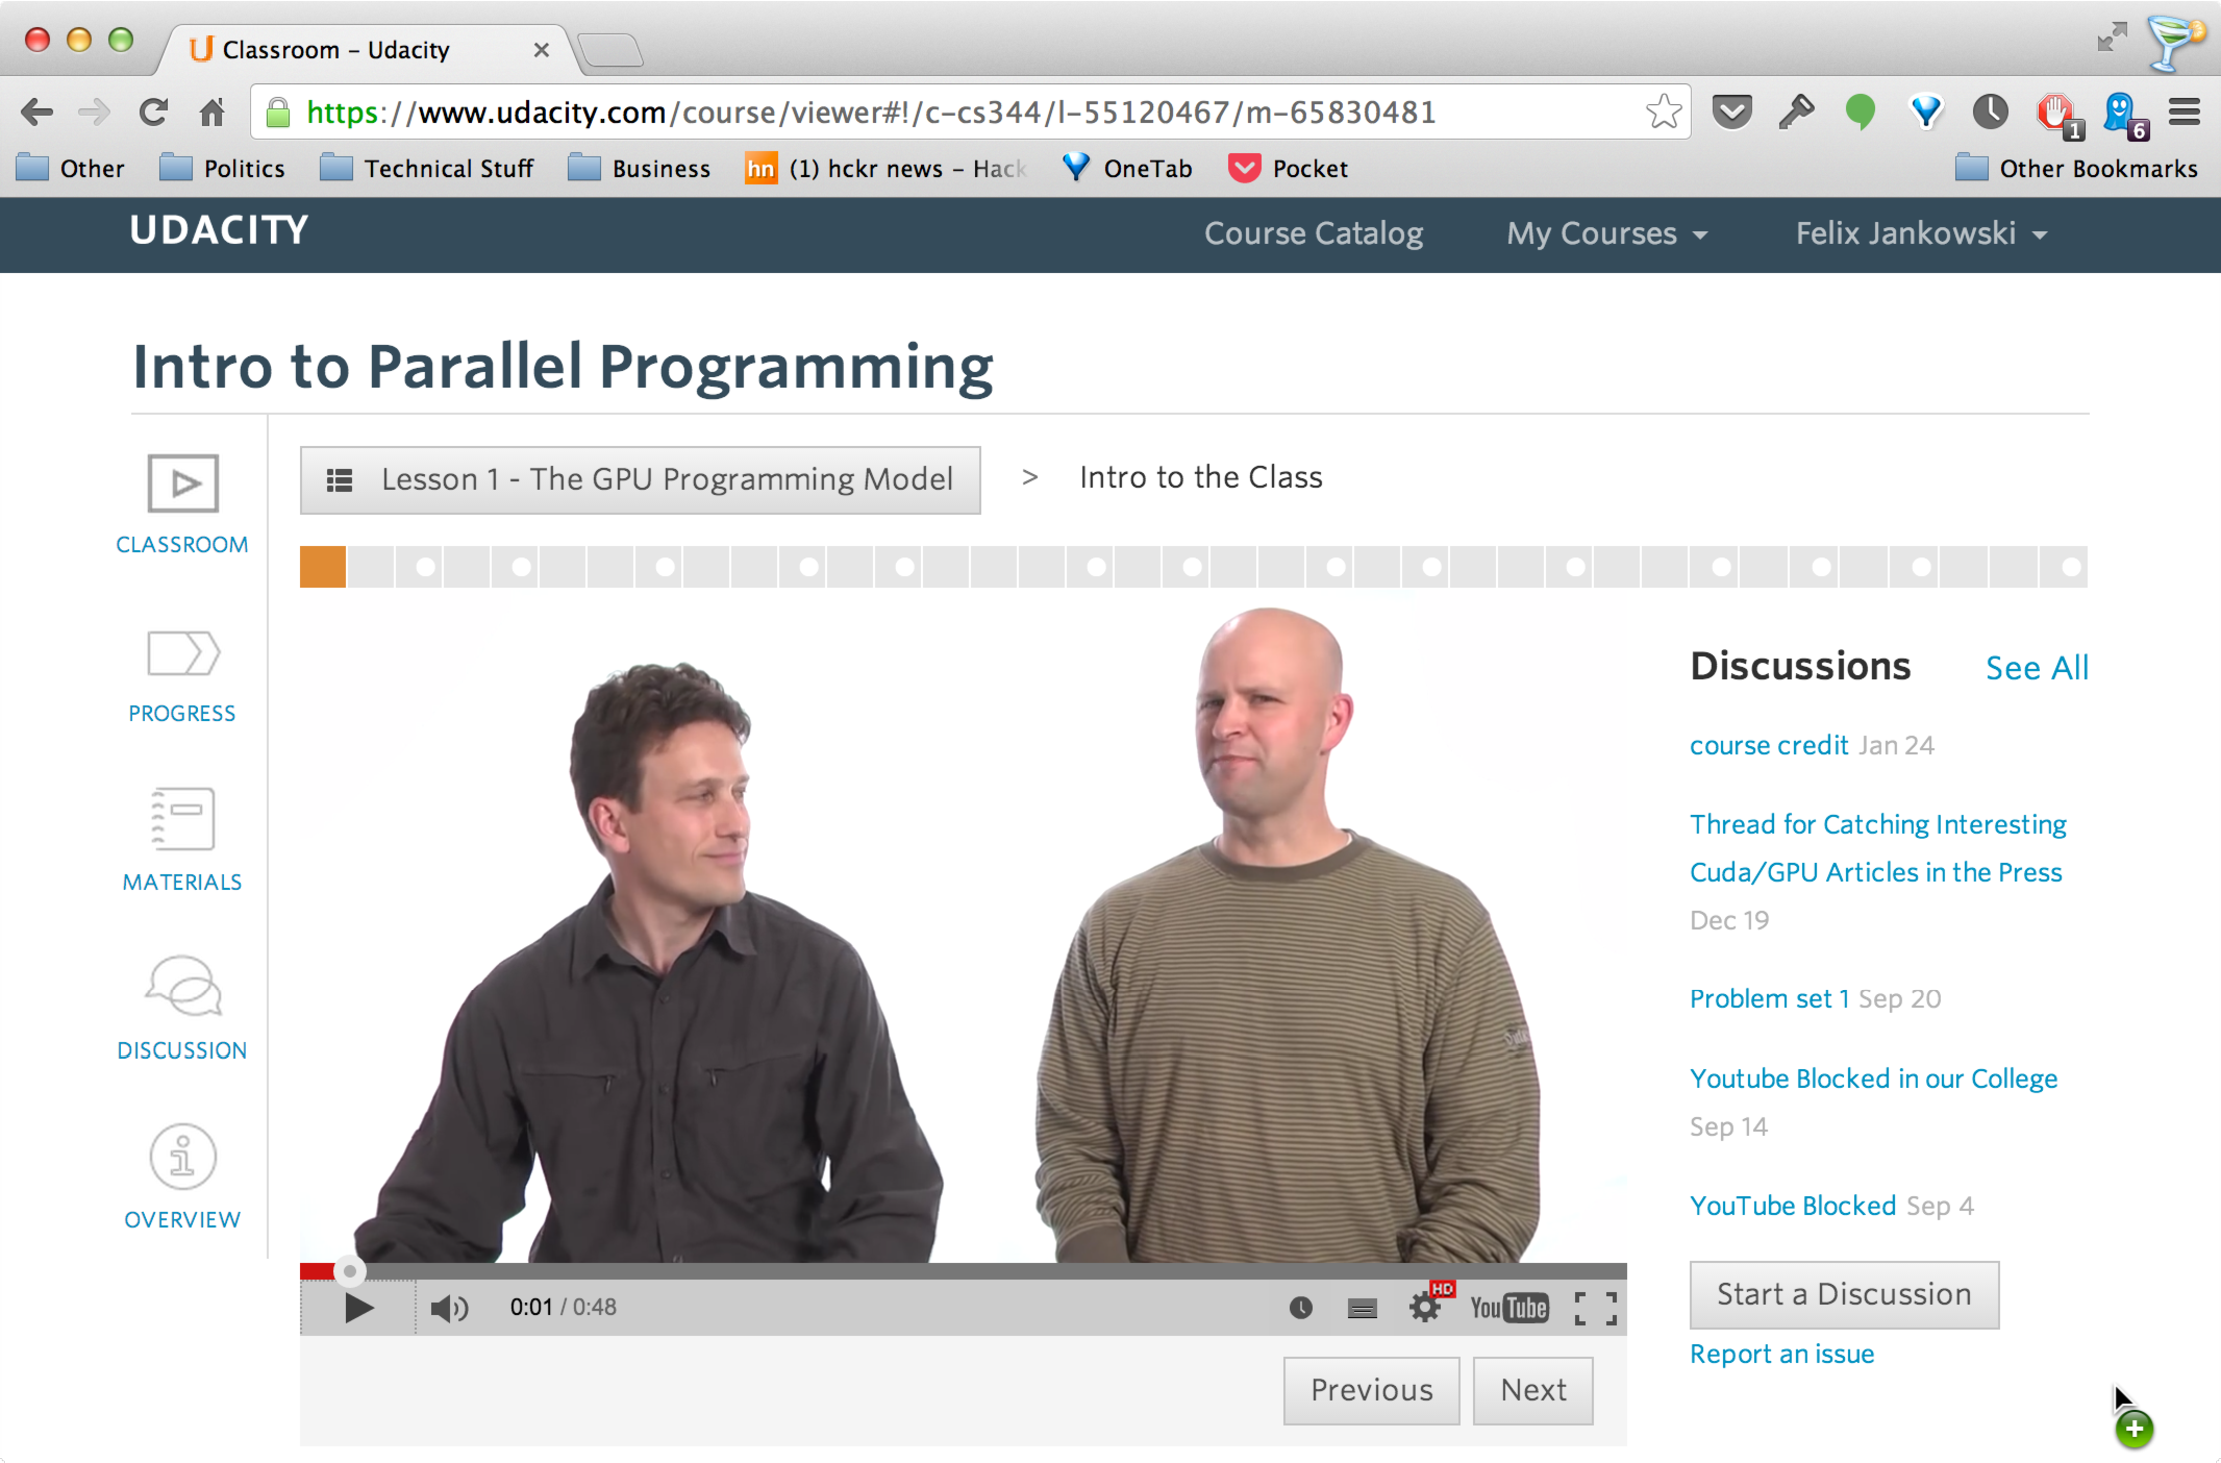
\includegraphics[width=\textwidth]{img/udacity}
					\caption{Benutzeroberfläche von Udacity}
					\label{fig:screenshot-udacity}
				\end{center}
			\end{figure}


			Nach wie vor liegt der Fokus des Angebots in erster Linie auf dem Bereich Informatik, mittlerweile werden aber auch Kurse in anderen Fachbereichen, z.B. "`Intro to the Design of Everyday Things"' von Don Norman oder "`How to Build a Startup"' angeboten.

			Besonderes Merkmal von Udacity ist, dass die Teilnehmer nach Abschluss der Lehrveranstaltungen eine Prüfung ablegen können und dafür ein Zeugnis erhalten.
			Dies wird zum Teil über Firmenkooperationen (z.B. SalesForce) angeboten, bei denen die Teilnehmer eine offizielle Zertifizierung für das jeweilige Produkt erwerben.

			Neuerdings wird in Kooperation mit der Georgia Tech University ein vollständiger Masterstudiengang in Computer Science angeboten.
			Dies ist für besonders für amerikanische Studenten attraktiv, da diese einen offiziellen akademischen Grad erwerben, ohne die zum Teil horrenden Studiengebühren in voller Höhe tragen zu müssen.

		\subsection{Coursera}

		Kein Wissen über User
		keine Live-Experimente wie Instantlab
		
		Neugikeit: Instanz auf Knopfdruck
		
%%%%%%%%%%%%%%%%%%%%%%%%%%%%%%%%%%%%%%%%%%%%%%%%%%%%%%%%%%%%%%%%%%%%%%%%%%%%%%%%%%%%%%%%%%%%%%%%%%%%%%%%%
\section{Technologien}
\label{sec:technologies}
%%%%%%%%%%%%%%%%%%%%%%%%%%%%%%%%%%%%%%%%%%%%%%%%%%%%%%%%%%%%%%%%%%%%%%%%%%%%%%%%%%%%%%%%%%%%%%%%%%%%%%%%%

		Allgemeines zur Plattform und zur Virtualisierung

		Plattform Intel x86 / Microsoft wegen der durchgängigen Unterstützung. \cite{PopekGoldberg}

		Spezialfälle: Binary rewriting, manche Operationen schneller in Softwre als in Hardware

		Warum ist Intel problematisch??

		Typ 1/2 Virtualisierung (hier ggf. nicht relevant)


		%%%%%%%%%%%%%%%%%%%%%%%%%%%%%%%%%%%%%%%%%%%%%%%%%%%%%%%%%%%%
		\subsection{VMWare}
		%%%%%%%%%%%%%%%%%%%%%%%%%%%%%%%%%%%%%%%%%%%%%%%%%%%%%%%%%%%%

		Relevanz: Feld eröffnet, große Menge Hardware

		%%%%%%%%%%%%%%%%%%%%%%%%%%%%%%%%%%%%%%%%%%%%%%%%%%%%%%%%%%%%
		\subsection{KVM}
		%%%%%%%%%%%%%%%%%%%%%%%%%%%%%%%%%%%%%%%%%%%%%%%%%%%%%%%%%%%%

		Relevanz: Standard reportoire, Open Source

		